\section{Umsetzung}

\subsection{Technologieentscheidung}
\subsubsection{Versuchssystem}\label{sec:TechnologieVersuchssystem}
\subsubsection{Demosystem}
Für die Technologieentscheidung muss zunächst zwischen den zwei Komponenten Client und Server unterscheiden werden.
Da für beide Teile unterschiedliche Anforderungen erfüllt werden müssen, erfolgt die Technologieentscheidung separat.
Außerdem findet eine Festlegung des verwendeten Protokolls für die Schnittstellenkommunikation statt.

\paragraph{Client}
Die grundlegende Anforderung an den Client ist die Umsetzung als Webapplikation.
Daraus leiten sich in erster Linie vier verschiedene Programmiersprachen ab: JavaScript/Type\-Script, Python, PHP und Ruby.

Für eine weitergehende Einschränkung ist der vorausgesetzte Funktionsumfang relevant.
Dieser ist sehr gering, da lediglich Input-Elemente für die Angabe eines zu authentifizierenden Sprechers, sowie zur Auswahl einer zu verwendeten Datei bereitgestellt werden müssen.
Außerdem muss eine Verbindung zu einem Back-End (Server) aufgebaut werden können.

Da diese Anforderungen durch alle vier Kandidaten erfüllt werden, muss die Entscheidung durch andere Kriterien erfolgen.
Hierbei spielen vor allem zwei Aspekte eine Rolle.
Eine Umfrage von Stack Overflow aus dem Jahr 2020 zeigt, dass JavaScript die beliebteste Programmiersprache von professionellen Entwickler ist.
Moderne Frameworks wie Reactjs und Angular haben die klassische Webprogrammierung in PHP über die letzten Jahre abgelöst \autocite[vgl.][]{stack_overflow_stack_nodate}.

Da es sich außerdem um ein Demosystem handelt, welches lediglich die Ergebnisse dieser Arbeit präsentieren soll und somit nicht in einem produktiven Umfeld betrieben wird, spielt die Technologieentscheidung nur eine untergeordnete Rolle.
Die Kompetenzen des Entwicklerteams liegen vor allem im Bereich der React Programmierung mit JavaScript beziehungsweise TypeScript.

Zusammenfassend fällt die Technologieentscheidung für die Client Implementierung somit auf das JavaScript Framework Reactjs in Kombination mit TypeScript.
TypeScript ermöglicht dabei gegenüber JavaScript die Verwendung von Datentypen, wodurch Datentypfehler im Rahmen der Implementierung vermieden werden können.

\paragraph{Schnittstelle}
Im Web-Umfeld spielt das \ac{HTTP} eine besondere Rolle.
Dabei handelt es sich um ein zustandsloses Protokoll zur Übertragung von Daten auf der Anwendungsschicht.
Ein Anwendungsfall ist dabei die Anfrage von Websiten im Browser über die URL.
Dazu wird eine sogenannte \ac{HTTP}-GET Anfrage an den Zielserver gesendet, welcher anschließend mit der angeforderten Ressource antwortet.

Nach demselben Prinzip kann das HTTP Protokoll ebenfalls dazu verwendet werden, eine Kommunikation zwischen Client und Server zu ermöglichen.
Die zu übergebenden Variablen des Clients an den Server können dabei innerhalb der URL des GET-Requests übertragen werden.
Gleichzeitig können die Ergebnisse des Servers beispielsweise im JSON-Format an den Client zurückgesendet werden.

Da das HTTP Protokoll somit alle benötigten Anforderungen erfüllt, kommt es für die Schnittstellenkommunikation zum Einsatz.

\paragraph{Server}
Für den Authentifizierungsprozess implementiert der Server denselben Ablauf wie das Versuchssystem.
Um eine doppelte Entwicklung zu vermeiden, entsteht somit eine Abhängigkeit zwischen der Technologieentscheidung des Versuchssystems und des Servers.
Aus der Technologieentscheidung des Versuchssystems in Kapitel~\ref{sec:TechnologieVersuchssystem} geht die Programmiersprache Python hervor.
Somit sollte zunächst geprüft werden, ob die Anforderungen des Servers in der Sprache Python umsetzbar sind.

Neben dem Authentifizierungsprozess spielt ausschließlich die Schnittstellenkommunikation zwischen Client und Server eine Rolle für die Technologieentscheidung des Servers.
Da als Kommunikationsprotokoll HTTP eingesetzt wird, muss also eine Bibliothek gefunden werden, die die Verwendung dieses Protokolls in Python ermöglicht.
Hierzu kann Flask verwendet werden.

Bei Flask handelt es sich um ein Web Framework, welches eine Bereitstellung von \ac{API} Endpunkten, die über das \ac{HTTP} Protokoll abrufbar sind, ermöglicht.

Somit können alle Anforderungen an die Serverapplikation mittels der Programmiersprache Python umgesetzt werden.
Dazu können die bereits entwickelten Komponenten für den Authentifizierungsprozess aus dem Versuchssystem übernommen werden.

\subsection{Versuchssystem}
\subsection{Demosystem}
Die Umsetzung von Client und Server ist im Folgenden kurz beschrieben.
Dabei werden lediglich die wichtigsten Aspekte benannt.
Da der Authentifizierungsablauf bereits im vorangehenden Kapitel erläutert wurde, wird in der Umsetzung des Servers nicht mehr darauf eingegangen.

\paragraph{Client}
Die im Client implementierte Benutzeroberfläche zeigt eine Login-Abfrage (siehe Abbildung~\ref{fig:AppLogin}).
Diese unterteilt sich in zwei Abschnitte.
Zunächst kann über ein Eingabefeld die ID des zu authentifizierenden Nutzers angegeben werden.
Anschließend kann eine zu verwendende Audiodatei aus einer Liste ausgewählt werden.
Dabei stehen für jeden Nutzer mindestens fünf verschiedene Dateien zur Verfügung.
Um die Benutzerfreundlichkeit zu verbessern besteht dabei zusätzlich die Möglichkeit, die ausgewählte Datei im Browser abzuspielen.
Dafür wird der HTML \textFunktion{<audio>} tag verwendet.
\begin{figure}[H]
    \begin{subfigure}[c]{0.49\textwidth}
        \centering
        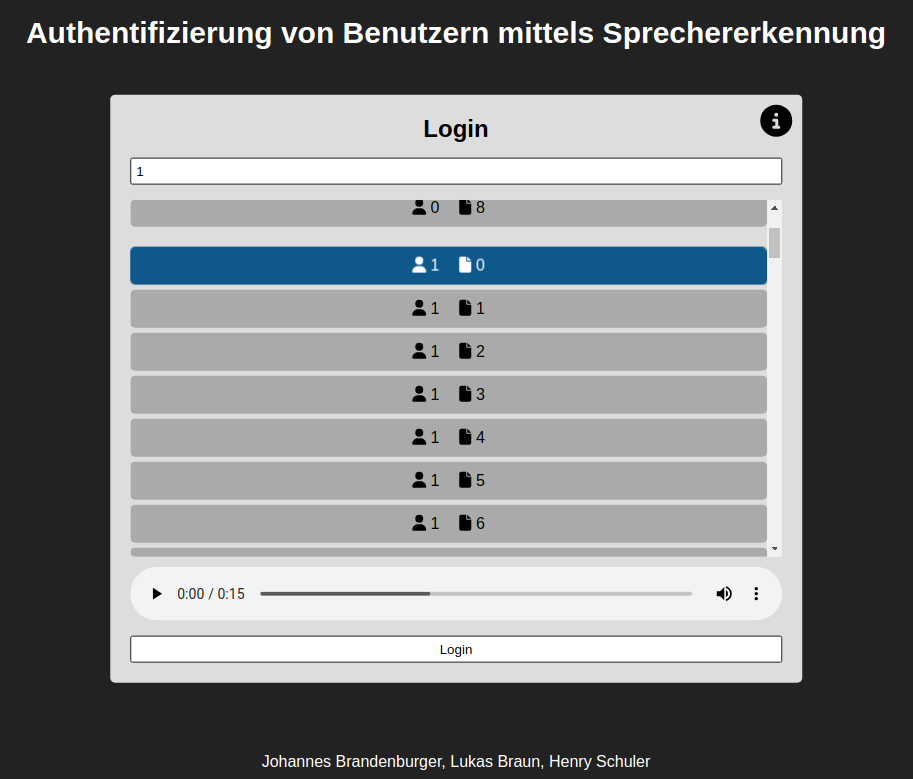
\includegraphics[width=0.9\textwidth, keepaspectratio]{images/UI.png}
        \subcaption{App/Login}
        \label{fig:AppLogin}
    \end{subfigure}
    \begin{subfigure}[c]{0.49\textwidth}
        \centering
        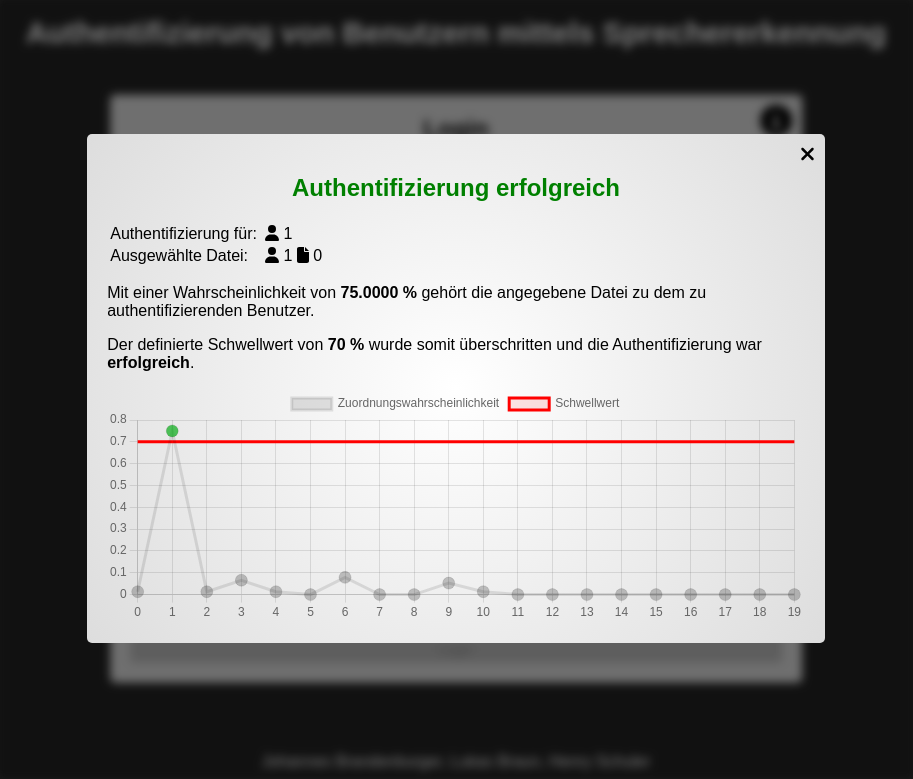
\includegraphics[width=0.9\textwidth, keepaspectratio]{images/UIResult.png}
        \caption{Result}
        \label{fig:Result}
    \end{subfigure}
    \caption{Weboberfläche}
\end{figure}
Über den Login-Knopf wird die Authentifizierungsanfrage an den Server gesendet.
Dafür wird die \textFunktion{fetch()} Funktion von JavaScript verwendet.
Die zu übergebenden Parameter werden als URL-Parameter angegeben.

Die Darstellung des Ergebnisses mittels der \textKlasse{Result} Komponente ist in Abbildung~\ref{fig:Result} dargestellt.
Dem Benutzer werden sowohl seine Authentifizierungsangaben, als auch das Ergebnis der Authentifizierung in Textform angezeigt.
Die Klassifikation als \gqq{erfolgreich} oder \gqq{fehlgeschlagen} kann sowohl dem Text als auch der Farbe der Überschrift (grün oder rot) entnommen werden.

Zusätzlich erhält der Benutzer einen grafischen Einblick in die Wahrscheinlichkeitsverteilung der Zuordnung der ausgewählten Sprecherdatei zu den verschiedenen Sprechern.
Das Diagramm wird mit Hilfe der Bibliotheken chart.js und react-chartjs-2 eingebunden.

\paragraph{Server} 
Wie in der Technologieentscheidung bereits erwähnt, wird der Server mit Hilfe der Bibliothek Flask implementiert.
Listing~\ref{lst:serverPy} zeigt dabei die wesentlichen Codeabschnitte für die Umsetzung des Servers als Flask Applikation.
\begin{lstlisting}[language=Python,numbers=none,caption=Ausschnitt server.py,label=lst:serverPy]
    app = Flask(__name__)
    CORS(app)

    @app.route("/", methods=["GET", "POST"])
    def handle_api_request():
        ...

    if __name__ == '__main__':
        app.run(debug=False, host='127.0.0.1', port=5500)
\end{lstlisting}
Zunächst muss eine neue Flask \textVariable{app} erstellt werden.
Mittels \textFunktion{CORS(app)} wird dabei sichergestellt, dass eine Verbindung zwischen Client und Server trotz unterschiedlichem Ursprung möglich ist.

Die Authentifizierungsfunktion wird über die Wrapper-Funktion \textFunktion{handle\_api\_request()} und dem Decorator \textFunktion{@app.route()} als \ac{API} Endpoint verfügbar gemacht.

Abschließend kann der Server über die Anweisung \textFunktion{app.run()} unter Angabe der IP-Adresse und des Ports gestartet werden.